\section{Производная}
\epigraph{\textsf{Your focus determines your reality}}{\texttt{Qui-Gon Jinn}}
Так как с понятием функции мы уже познакомились, а также обсудили различные виды функций, то можно приступать к их анализу. Например, мы хотим узнать насколько сильно меняется значение какой либо физической величины в какой-либо точке. Прекрасным примером для анализа этого может служить координата.
\subsection{Я-скорость, кчау}
Пускай Рома Лисин бежит за школьниками в игре "охота на кабанчиков". Зададим его положение функцией $z(t)$ в момент времени $t$. В момент времени $t + \Delta t$ он прибежал в точку $z(t + \Delta t)$, где $\Delta t > 0$.
Тогда \textbf{средняя скорость} на отрезке времени $[t, t + \Delta t]$ определяется как:
\begin{equation*}
    \bar{v} (t, t + \Delta t) = \frac{z(t + \Delta t) - z(t)}{\Delta t} = \frac{\Delta z}{\Delta t}
\end{equation*}
Где назовем $\Delta z$ \textbf{приращением координаты $z$}. Теперь если мы устремим $\Delta t$ к нулю, фиксируя $t$, то есть запишем это как $\Delta t \rightarrow 0$, тогда получим долгожданную \textbf{мгновенную скорость}.
\begin{definition}
    \textbf{Мгновенная скорость} в момент времени $t$ - это 
    \begin{equation*}
        z^{'}(t) = \frac{dz}{dt} = \lim_{\Delta t \rightarrow 0} \frac{z(t + \Delta t) - z(t)}{\Delta t} = \lim_{\Delta t \rightarrow 0} \frac{\Delta z}{\Delta t}
    \end{equation*}
    то есть отношение пути, пройденного за бесконечно малый промежуток времени, к величине этого промежутка с учетом знака.
\end{definition}
Зачастую производные каких-любо функций от времени принято обозначать с точкой наверху: $\dot{z}$. Нетрудно установить, что если $\dot{z} < 0$, то Рома бежит в сторону уменьшения координаты $z$, если же $\dot z > 0$ - в сторону увеличения.

\begin{example}
    Равномерное движение
    \begin{equation*}
        z(t) = z_0 + vt
    \end{equation*}
    тогда $\displaystyle\dot{z} = \lim_{\Delta t \rightarrow 0} \frac{z_0 + v(t + \Delta t) - z_0 - vt}{\Delta t} = v = const$ - постоянная величина.
\end{example}

\subsection{Бесконечность не предел!}
Углубимся в определение предела. Предельные соотношения не обязательно искать при уменьшении параметра к $0$ или увеличении к $\infty$. Например, значения функции $y = x^2$ в точке $x = 5$ можно также записать через предел
\begin{equation*}
    y|_{x = 5} = \lim_{x \rightarrow 5} x^2 = 5^2 = 25
\end{equation*}
Если сильно хочется всегда брать пределы при стремлении к $0$, то можно просто сделать замену $x \rightarrow \xi = x - x_0$, где $x_0$ - то значение, к которому мы стремимся.
\begin{definition}
    \textbf{Предел} функции $f(x)$ в точке $x_0$ - это 
    \begin{equation*}
        f(x)|_{x = x_0} = \lim_{x \rightarrow x_0} f(x) = \lim_{\xi \rightarrow 0} f(\xi + x_0) = f(x_0)
    \end{equation*}
\end{definition}
Если же необходимо найти предел на $\infty$, это также можно сделать, совершив замену $x \rightarrow \zeta = 1/x$.
\begin{example}
    Найдем предел при $x \rightarrow \infty$ для функции $y = \bigl(\frac{2}{3} \bigr)^x$
    \begin{equation*}
        \lim_{x \rightarrow \infty} \bigl( \frac{2}{3}\bigr)^x = 0
    \end{equation*}
\end{example}

\subsection{Основные свойства производной}
Для того, чтобы двигаться дальше, необходимо обсудить производные от композиции двух функций.
\begin{itemize}
    \item \textbf{Производная суммы/разности}
    \begin{equation*}
        (f \pm g)^{'} = \lim_{\Delta x \rightarrow 0} \frac{f(x + \Delta x) - f(x) \pm g(x + \Delta x) - g(x)}{\Delta x} = f^{'} \pm g^{'}
    \end{equation*}
    \item \textbf{Производная произведения}
    \begin{multline*}
        (fg)^{'} = \lim_{\Delta x \rightarrow 0} \frac{f(x + \Delta x)g(x + \Delta x) - f(x)g(x)}{\Delta x} = \\
        =\lim_{\Delta x \rightarrow 0} \frac{(\Delta f + f(x))(\Delta g + g(x)) - f(x)g(x)}{\Delta x} = \\
        = \lim_{\Delta x \rightarrow 0} \frac{\Delta f g(x) + \Delta g f(x)}{\Delta x} = f^{'}g + g^{'} f
    \end{multline*}
    \item \textbf{Производная частного}
    \begin{multline*}
        \bigl(\frac{f}{g} \bigr)^{'} = \lim_{\Delta x \rightarrow 0} \frac{\frac{f(x + \Delta x)}{g(x + \Delta x)} - \frac{f(x)}{g(x)}}{\Delta x} = \lim_{\Delta x \rightarrow 0} \frac{(\Delta f + f(x))g(x) - (\Delta g + g(x))f(x)}{\Delta x (\Delta g + g(x)) g(x)} =\\
        = \lim_{\Delta x \rightarrow 0} \frac{\frac{\Delta f}{\Delta x} g - \frac{\Delta g}{\Delta x} f}{g^2} = \frac{f^{'} g - g^{'} f}{g^2}
    \end{multline*}
    \item \textbf{Производная сложной функции}
    \begin{multline*}
        (f(g(x)))^{'} = \lim_{\Delta x \rightarrow 0} \frac{f(g(x + \Delta x)) - f(g(x))}{\Delta x} = \lim_{x \rightarrow 0}\frac{f(g + \Delta g) - f(g)}{\Delta g}\ \frac{\Delta g}{\Delta x} = \frac{df}{dg}\ \frac{dg}{dx} =\\
        = [f(g)]^{'}_{g} g^{'}
    \end{multline*}
    \item \textbf{Производная обратной функции}
    Потребуем только, чтобы $y=f(x)$ была строго монотонной, то есть если $x_2 > x_1$, то $f(x_2) > или < f(x_1)$. Так как между $x$ и $f$ есть однозначное соответствие, то можно ввести функцию $x = g(y)$, то $\Delta x \rightarrow 0 \Rightarrow \Delta y \rightarrow 0$ и наоборот. Тогда 
    \begin{equation*}
        g^{'}(y) = \lim_{\Delta y \rightarrow 0} \frac{\Delta x}{\Delta y} = \lim_{\Delta y \rightarrow 0} \frac{1}{\frac{\Delta y}{\Delta x}} =\lim_{\Delta x \rightarrow 0} \frac{1}{\frac{\Delta y}{\Delta x}} = \frac{1}{f^{'}(x)}
    \end{equation*}
\end{itemize}
Укажем \textbf{геометрический смысл} производной: если нарисовать график функции $z=z(t)$, то $\dot{z} = \tan \alpha$, где $\alpha$ — угол наклона касательной, проведённой к графику в точке $(t, z(t))$, к оси $t$.
\begin{example}
    Равноускоренное движение
    \begin{equation*}
        z(t) = z_0 + v_0t + \frac{at^2}{2}
    \end{equation*}
    Тогда легко получить $\dot{z}= v_0 + at,\ \ddot{z} = a$, где $v_0$ - начальная скорость, $a$ - ускорение.
\end{example}
\begin{prac}
    Получи, что $(t^{n})^{'} = n t^{n-1},\ \forall n \in \mathbb{N}$ (подсказка\footnote{воспользуйся методом индукции})
\end{prac}
\begin{prac}
    Найди производную функции $f(x) = \arctg x$.
\end{prac}

\subsection{Число $e$. Второй замечательный предел.}
Когда мы уже разобрались с тем, что такое производная, то следует поговорить про примечательную функцию, с которой эта производная связана.

Предположим, что мы нажли функцию вида $y = a^x$ производная у которой равна самой же функции, то есть
\begin{equation*}
    y^{'} = y
\end{equation*}
Пусть это происходит при $a = e$. Так как наше выражение должно быть верно в нуле, тогда
\begin{equation*}
    (e^x)^{'}|_{x = 0} = 1 \Rightarrow \lim_{\Delta x \rightarrow 0} \frac{e^{\Delta x} - 1}{\Delta x} = 1
\end{equation*}
Положим $\Delta x = \frac{1}{n},\ n\gg 1$, тогда с большой точностью получим $e^{\Delta x} \approx 1 + \Delta x$, где формула точнее с уменьшением $\Delta x$. При $n \in \mathbb{Z}$ имеем
\begin{equation*}
    e = (e^{1/n})^{n} \approx (1 + \frac{1}{n})^{n}
\end{equation*}
\begin{theorem}
    \textbf{Второй замечательный предел}
    \begin{equation*}
        e = \lim_{n \rightarrow \infty} \bigl(1 + \frac{1}{n}\bigr)^{n}
    \end{equation*}
\end{theorem}

\subsection{Первый замечательный предел}
Сразу же запишем исследуемый предел
\begin{equation*}
    \lim_{x \rightarrow 0} \frac{\sin x}{x}
\end{equation*}
Для пруфа этого утверждения посмотрим необходимый геометрический рисунок. 
\begin{figure}[h!]
    \centering
    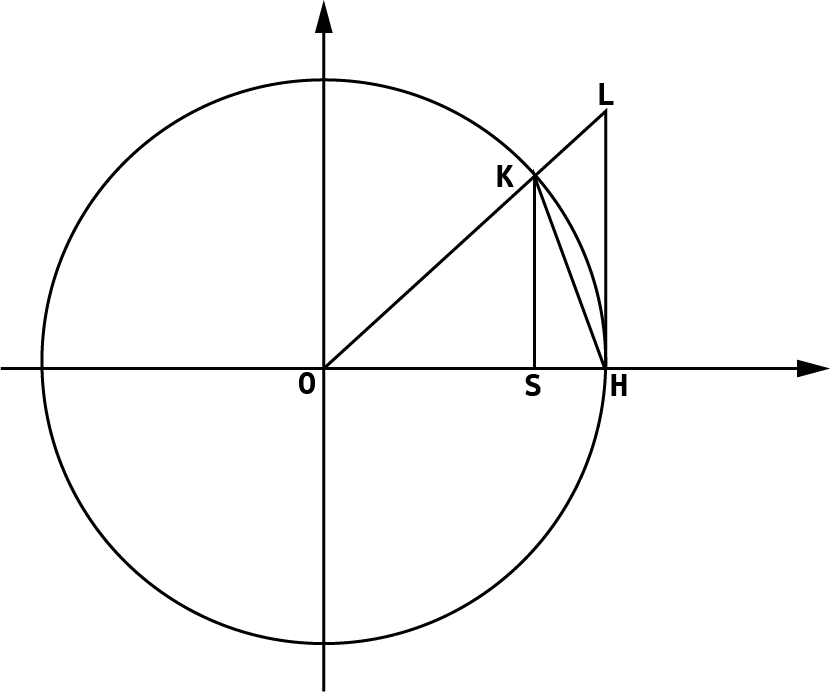
\includegraphics[scale=0.5]{pics/first_great_lim.png}
    \caption{Первый замечательный предел}
\end{figure}

Очевидно, что
\begin{equation*}
    S_{\Delta OKH} < S_{\text{сектор}\ OKH} < S_{\Delta OLH}
\end{equation*}
Площади треугольников соответственно: $S_{\Delta OKH} = \frac{\sin x}{2}$, $S_{\text{сектор}\ OKH} = \frac{x}{2}$, $S_{\Delta OLH} = \frac{\tan x}{2}$. Таким образом
\begin{equation*}
    \frac{\sin x}{x} < \frac{x}{2} < \frac{\tan x}{2} \Rightarrow 1 > \frac{\sin x}{x} > \frac{1}{\cos x}
\end{equation*}
Переходя к пределу
\begin{equation*}
    1 \geq \lim_{x \rightarrow 0} \frac{\sin x}{x} \geq \lim_{x \rightarrow 0} \frac{1}{\cos x} = 1
\end{equation*}
Таким образом
\begin{theorem}
    \textbf{Первый замечательный предел}
    \begin{equation*}
        \lim_{x \rightarrow 0}\ \frac{\sin x}{x} = 1
    \end{equation*}
\end{theorem}